\section{Unit 7}
\subsection{Lecture 26: Diagonalization of Symmetric Matrices [7.1]}

\begin{defbox}{Symmetric Matrices}{}
    A \textbf{symmetric matrix} is a matrix $A$ such that $A^{T}=A$. Such a matrix is necessarily square (i.e. all symmetric matrices are square). Its main diagonal entries are arbitary, but its other entries occur in pairs - on opposite sides of the main diagonal. 
\end{defbox}

\begin{thm}{}{\label{thm:7.1}}
   If $A$ is symmetric then any two eigenvectors from different eigenspaces are orthogonal. 
\end{thm}

\begin{defbox}{Orthogonally Diagonalizable Matrices}{}
    An $n\times\,n$ matrix $A$ is said to be \textbf{orthogonally diagonalizable} if there an orthogonal matrix $P$ (with $P^{-1} = P^{T}$) and a diagonal matrix $D$ such that 
    \[ A = PDP^{T} = PDP^{-1} \]
\end{defbox}

It is worth noting that for $A$ to be orthogonally diagonalizable, $A$ must have $n$ linearly independent and orthonormal eigenvectors. This is only possible when $A$ is symmetric since if $A$ is symmetric then 
\[ A^{T} = (PDP^{T})^{T} = P^{TT}D^{T}P^{T} = PDP^{T} = A. \]
In fact, $A$ being symmetric is both necessary and sufficient for $A$ being orthogonally diagonalizable. 

\begin{thm}{}{}
    An $n\times\,n$ matrix $A$ is orthogonally diagonalizable if, and only if, $A$ is a symmetric matrix. 
\end{thm}

\begin{example}{}{}
    Orthogonally diagonalize the matrix $A$ below, with the characteristic equation $0 = -\lambda^3 + 12\lambda^2 - 21\lambda - 98 = -\left(\lambda-7\right)^2\left(\lambda+2\right)$. 
    \[
        A = \begin{pmatrix}
            3 & -2 & 3 \\
            -2 & 6 & 2 \\
            4 & 2 & 3
        \end{pmatrix} 
    \]
    \begin{solution}
        We can solve the given characteristic equation to find the $\lambda = 7$ (with multiplicity 2) and $\lambda = -2$. We must find the eigenvectors of $A$ in order to form the orthogonal matrix $P$. For $\lambda = 7$ we have eigenvectors 
        \[
            \vec{v}_1 = \begin{pmatrix}
                1 \\ 0 \\ 1
            \end{pmatrix}, 
            \quad \vec{v}_2 = \begin{pmatrix}
                -1/2 \\ 1 \\ 0
            \end{pmatrix}
        \]
        and for $\lambda = -2$ we have 
        \[
            \vec{v}_3 = \begin{pmatrix}
                -1 \\ -1/2 \\ 1
            \end{pmatrix}
        \]
        However, recall from earlier that for $A$ to be orthogonally diagonalizable we must have $n$ linearly independent and orthogonal vectors, and while $\vec{v}_1$ and $\vec{v}_2$ are linearly independent, they are not orthogonal. We can use the Gram-Schmidt process~(\ref{thm:gram}) to turn the basis for our eigenspace into an othogonal basis: 
        \begin{align*}
            \vec{z_1} &= \vec{v_1} \\
            \vec{z_2} &= \vec{v_2} - \frac{\vec{v_2}\cdot\vec{z_1}}{\vec{z_1}\cdot\vec{z_1}}\vec{v_1} = \begin{pmatrix}
                -1/2 \\ 1 \\ 0 
            \end{pmatrix}
            - \frac{-1/2}{2}\begin{pmatrix}
                1 \\ 0 \\ 1
            \end{pmatrix}
            = \begin{pmatrix}
                -1/4 \\ 1 \\ 1/4
            \end{pmatrix}
        \end{align*}
        Now that $\braces{\vec{z_1}, \vec{z_1}}$ is an orthogonal set, we can form an orthonormal set $\braces{\vec{u_1}, \vec{u_2}, \vec{u_3}}$ with 
        \[
            \vec{u_1} = \begin{pmatrix}
                1/\sqrt{2} \\ 0 \\ 1/\sqrt{2}
            \end{pmatrix}, 
            \quad \vec{u_2} = \begin{pmatrix}
                -1/\sqrt{18} \\ 4/\sqrt{18} \\ 1/\sqrt{18}
            \end{pmatrix}, 
            \quad \vec{u_3} = \begin{pmatrix}
                -2/3 \\ -1/3 \\ 2/3
            \end{pmatrix}
        \]
        where $\vec{u_1}, \vec{u_2},$ and $\vec{u_3}$ are $\vec{z_1}, \vec{z_2},$ and $2\vec{v_3}$ normalized. Using Theorem~(\ref{thm:7.1}) we can form the orthonormal set $\braces{\vec{u_1}, \vec{u_2}, \vec{u_3}}$ and use it to make $P$ (along with using $\lambda=7, 7, -2$) and $D$
        \[
            P = \begin{pmatrix}
                1/\sqrt{2} & -1/\sqrt{18} & -2/3 \\
                0 & 4/\sqrt{18} & -1/3 \\
                1/\sqrt{2} & 1/\sqrt{18} & 2/3
            \end{pmatrix}, 
            \quad D = \begin{pmatrix}
                7 & 0 & 0 \\
                0 & 7 & 0 \\
                0 & 0 & -2
            \end{pmatrix}
        \]
        Thus, we have found $P$ and $D$ such that $A=PDP^{-1}=PDP^{T}$.
    \end{solution}

\end{example}

\begin{thm}{}{}
    An $n\times\,n$ symmetric matrix $A$ has the following properties:
    \begin{enumerate}
        \item $A$ has $n$ \textbf{real} eigenvalues, counting multiplicity
        \item The dimension of each eigenspace for each eigenvalue $\lambda$ equals the multiplicity of $\lambda$ as a root of the characteristic equation 
        \item The eigenspaces are mutually orthogonal (in the sense that eigenvectors corresponding to different eigenvalues are orthogonal)
        \item $A$ is orthogonally diagonalizable
    \end{enumerate} 
\end{thm}

\newpage 

\begin{impbox}{Spectral Decomposition}{}
    Suppose $A = PDP^{-1}$, where the columns of $P$ are orthonormal eigenvectors $\vec{u}_1, \ldots, \vec{u_n}$ of $A$ and the corresponding eigenvalues $\lambda_1, \ldots, \lambda_n$ are in the diagonal matrix $D$. Then, since $P^{-1} = P^{T}$, 
    \begin{align*}
        A &u= PDP^{T} = \begin{pmatrix}
            \left(\vec{u}_1\right) & \cdots & \left(\vec{u}_n\right)
        \end{pmatrix}
        \begin{pmatrix}
            \lambda_1 & \cdots & 0 \\
            \vdots & \ddots & \\
            0 & & \lambda_n
        \end{pmatrix}
        \begin{pmatrix}
            \vec{u_1}^{T} \\
            \vdots \\
            \vec{u_n}^{T}
        \end{pmatrix} \\
        &= \begin{pmatrix}
            \left(\lambda_1\vec{u_1}\right) & \cdots & \left(\lambda_n\vec{u_n}\right)
        \end{pmatrix}
        \begin{pmatrix}
            \vec{u_1}^{T} \\
            \vdots \\
            \vec{u_n}^{T}
        \end{pmatrix}
    \end{align*}
    Expanding out this product gives, 
    \begin{equation}{\label{eq:7.1}}
        A = \lambda_{1}\vec{u_1}\vec{u_1}^{T} + \lambda_{2}\vec{u_2}\vec{u_2}^{T} + \cdots + \lambda_{n}\vec{u_n}\vec{u_n}^{T} 
    \end{equation}
    This representation of $A$ is called a \textbf{spectral decomposition} of $A$ because it breaks up $A$ into pieces determined by the spectrum (eigenvalues) of $A$. 
\end{impbox}

\begin{example}{}{}
    Construct a spectral decomposition of the matrix $A$ with the given orthogonal diagonalization, below 
    \[
        A = \begin{pmatrix}
            7 & 2 \\
            2 & 4
        \end{pmatrix} 
        = \begin{pmatrix}
            2/\sqrt{5} & -1/\sqrt{5} \\
            1/\sqrt{5} & 2/\sqrt{5}
        \end{pmatrix}
        \begin{pmatrix}
            8 & 0 \\
            0 & 3
        \end{pmatrix}
        \begin{pmatrix}
            2/\sqrt{5} & 1/\sqrt{5} \\
            -1/\sqrt{5} & 2/\sqrt{5}
        \end{pmatrix}
    \] 
    \begin{solution}
        Start by labeling the columns of $P$ as $\vec{u_1}$ and $\vec{u_2}$. Now, using the formula given by~(\ref{eq:7.1}), 
        \[
            A = 8\vec{u_1}\vec{u_1}^{T} + 3\vec{u_2}\vec{u_2}^{T} 
        \]
    \end{solution}
\end{example}

\subsection{Lecture 27: Quadratic Forms [7.2]}
\begin{defbox}{}{}
    A \textbf{quadratic form} on $\RR^{n}$ is a function $Q$ defined on $\RR^{n}$ whose value of a vector $\vec{x}$ in $\RR{n}$ can be computed an an expression of the form $Q\left(\vec{x}\right) = \vec{x}^{T}A\vec{x}$, where $A$ is an $n\times\,n$ symmetric matrix. The matrix $A$ is called the \textbf{matrix of the quadratic form}.
\end{defbox}

\begin{example}{}{}
    Let $\vec{x}=\left(\begin{smallmatrix} x_1 \\ x_2 \end{smallmatrix}\right)$ and find $\vec{x}^{T}A\vec{x}$ for $A$ below. 
    \[
        A = \begin{pmatrix}
            3 & -2 \\
            -2 & 7
        \end{pmatrix} 
    \]
    \begin{solution}
        \begin{align*}
            \vec{x}^{T}A\vec{x} &= \begin{pmatrix}
                x_1 & x_2
            \end{pmatrix}
            \begin{pmatrix}
                3 & -2 \\
                -2 & 7
            \end{pmatrix}
            \begin{pmatrix}
                x_1 \\ x_2
            \end{pmatrix} \\
            &= x_1\left(3x_1 - 2x_2\right) + x_2\left(-2x_1 + 7x_2\right) \\
            &= 3x_1^2 - 2x_{1}x_{2} - 2x_{1}x_{2} + 7x_{2}^{2} \\
            &= 3x_1^2 + 7x_2^2 - 4x_{1}x_{2}
        \end{align*}
    \end{solution}
\end{example}
Notice that in the above example that the coefficients of the quadratic terms ($x_1^2$ and $x_2^2$) are exactly the entries on the main diagonal of $A$. Next notice that the coefficients of the cross-product term ($x_{1}x_{2}$) is the sum of the entires at $(1, 2)$ and $(2, 1)$. In general, this holds true. The coefficients of a cross-product term $x_{i}x_{j}$ will always be twice the entries at $(i, j)$ and at $(j, i)$. 

\begin{example}{}{}
    For $\vec{x}\in\RR^{3}$, let $Q\left(\vec{x}\right) = 5x_1^2 + 3x_2^2 + 2x_3^2 - x_{1}x_{2} + 8x_{2}x_{3}$. Write this quadratic form as $\vec{x}^{T}A\vec{x}$.
    \begin{solution}
        Using the logic laid out in the paragrpah above, we can form the matrix $A$ quite easily to give: 
        \[
            \vec{x}^{T}A\vec{x} = \begin{pmatrix}
                x_1 & x_2 & x_3 
            \end{pmatrix}
            \begin{pmatrix}
                5 & -1/2 & 0 \\
                -1/2 & 3 & 4 \\
                0 & 4 & 2 
            \end{pmatrix}
            \begin{pmatrix}
                x_1 \\ x_2 \\ x_3
            \end{pmatrix}
        \]
    \end{solution}
\end{example}

\begin{impbox}{Change of Variable in a Quadratic Form}{}
    If $\vec{x}\in\RR^{n}$, then a \textbf{change of variables} is an equation of the form 
    \[
        \vec{x} = P\vec{y} 
    \]
    where $P$ is an invertible matrix and $\vec{y}\in\RR^{n}$. Here $\vec{y}$ is the coordinate vecotr of $\vec{x}$ relative to the basis of $\RR^{n}$ determined by the columns of $P$.
\end{impbox}

\begin{example}{}{}
    Make a change of varibales that transforms the quadratic form given by $Q\left(\vec{x}\right) = x_1^2 - 8x_{1}x_{2} - 5x_2^2$.
    \begin{solution}
        The matrix of the standard form $Q$ is 
        \[
            A = \begin{pmatrix}
                1 & -4 \\
                -4 & -5
            \end{pmatrix}.
        \]
        The reader can verify that for $A$ we have
        \[
            \lambda = 3: \begin{pmatrix}
                2/\sqrt{5} \\ -1/\sqrt{5}
            \end{pmatrix}, 
            \quad \lambda = -7: \begin{pmatrix}
                1/\sqrt{5} \\ 2/\sqrt{5}
            \end{pmatrix}
        \]
        Since $A$ is symmetric and these vectors belong to different eigenspaces, by Thereom~(\ref{thm:7.1}) they must be orthogonal. Thus, 
        \[
            P = \begin{pmatrix}
                2/\sqrt{5} & 1/\sqrt{5} \\
                -1/\sqrt{5} & 2/\sqrt{5}
            \end{pmatrix}, 
            \quad D = \begin{pmatrix}
                3 & 0 \\
                0 & -7
            \end{pmatrix}.
        \]
        So, $A = PDP^{-1} \Rightarrow D = P^{-1}AP = P^{T}AP$. If $\vec{x} = \left(\begin{smallmatrix} x_1 \\ x_2 \end{smallmatrix}\right)$ and $\vec{y} = \left(\begin{smallmatrix} y_1 \\ y_2 \end{smallmatrix}\right)$, then 
        \begin{align*}
            x_1^2 - 8x_{1}x_2 - 5x_2^2 &= \vec{x}^{T}A\vec{x} \\
            &= \left(P\vec{y}\right)^{T}A\left(P\vec{v}\right) \\
            &= \vec{y}^{T}P^{T}AP\vec{y} \\ 
            &= \vec{y}^{T}D\vec{y} \\
            &= 3y_1^2 - 7y_2^2
        \end{align*}
    \end{solution}
\end{example}

\begin{thm}{}{}
    The $A$ be an $n\times\,n$ symmetric matrix. Then there is an orthogonal change of variables $\vec{x} = P\vec{y}$, that transforms $\vec{x}^{T}A\vec{x}$ into a quadratic form $\vec{y}^{T}D\vec{y}$ with no cross-product term.
\end{thm}
The columns of $P$ are called the \textbf{principal axes} of the quadratic from $\vec{x}^{T}A\vec{x}$.

\begin{defbox}{Classifications of a Quadratic Form}{}
    A quadratic form $Q$ is 
    \begin{enumerate}
        \item \textbf{positive definite} if $\forall \vec{x}\neq\,0\,Q(\vec{x}) > 0$ 
        \item \textbf{negative definite} if $\forall \vec{x}\neq\,0\,Q(\vec{x}) < 0$ 
        \item \textbf{indefinite} if $Q(\vec{x})$ assumes both positive and negative values
    \end{enumerate}
\end{defbox}
We can also further classify $Q$ as \textbf{positive semidefinite} if $\forall \vec{x}\, Q(\vec{x}) \geq 0$ and \textbf{negative semidefinite} if $\forall \vec{x}\, Q\left(\vec{x}\right) \leq 0$.

\begin{thm}{}{}
    Let $A$ be an $n\times\,n$ symmetric matrix. Then a quadratic form $\vec{x}^{T}A\vec{x}$ is 
    \begin{enumerate}
        \item \textbf{positive definite} if, and only if, the eigenvaleus of $A$ are all positive
        \item \textbf{negative definite} if, and only if, the eigenvalues of $A$ are all negative
        \item \textbf{indefinite} if, and only if, the eigenvalues of $A$ are both positive and negative.
    \end{enumerate}
\end{thm}

A \textbf{positive definite matrix} $A$ is a symmetric m atrix for which the quadratic from $\vec{x}^{T}A\vec{x}$ is positive definite. There exist analagous definitions for negative definite, positive semidefinite, negative semidefinite, and indefinite.

\subsection{Lecture 28: Final Review}
\colorbox{red}{\underline{Practice Question 1:}} Find the orthogonal diagonalization of $A$ below such that $D=Q^{T}AQ$
\[
    A = \begin{pmatrix}
        4 & 2 & 2 \\
        2 & 4 & 2 \\
        2 & 2 & 4
    \end{pmatrix} 
\] 
\begin{solution}
    We start by finding the eigenvalues:
    \begin{align*}
        \det{A-\lambda I} =& \begin{vmatrix}
            4-\lambda & 2 & 2 \\
            2 & 4-\lambda & 2 \\
            2 & 2 & 4-\lambda 
        \end{vmatrix} \\
        \xrightarrow{R_1 \to R_1 - R_2}& \begin{vmatrix}
            2 - \lambda & \lambda - 2 & 0 \\
            2 & 4-\lambda & 2 \\
            2 & 2 & 4-\lambda
        \end{vmatrix} \\
        \xrightarrow{C_2 \to C_2 + C_1}& \begin{vmatrix}
            2-\lambda & 0 & 0 \\
            2 & 6-\lambda & 2 \\
            2 & 4 & 4-\lambda
        \end{vmatrix} \\
        =&\,(2-\lambda)((6-\lambda)(4-\lambda)-8) = 0 \\
        \Rightarrow&\,(2-\lambda)(\lambda^2-10\lambda+16) =(2-\lambda)(\lambda-2)(\lambda-8) \\
        \Rightarrow&\, \lambda_1 = 8, \lambda_2 = \lambda_3 = 2
    \end{align*}
    Next we can find the eigenvectors. For $\lambda_1=8$ we have: 
    \begin{align*}
        A - 8I = &\begin{pmatrix}
            -4 & 2 & 2 \\
            2 & -4 & 2 \\
            2 & 2 & -4 
        \end{pmatrix} 
        \xrightarrow[R_3 \to \frac{1}{2}R_3]{\frac{1}{2}R_1 \leftrightarrow \frac{1}{2}R_2} \begin{pmatrix}
            1 & -2 & 1 \\
            -2 & 1 & 1 \\
            1 & 1 & -2 
        \end{pmatrix} \\
        \xrightarrow[R_3 \to R_3 - R_1]{R_2 \to R_2 + 2R_1} &\begin{pmatrix}
            1 & -2 & 1 \\
            0 & -3 & 3 \\
            0 & 3 & -3 
        \end{pmatrix} 
        \xrightarrow{R_3 \to R_3 + R_2} \begin{pmatrix}
            1 & -2 & 1 \\
            0 & -3 & 3 \\
            0 & 0 & 0
        \end{pmatrix} \\
        \Rightarrow &\begin{cases}
            x_3 &= t \\
            x_2 &= t \\
            x_1 &= t
        \end{cases}
        \Rightarrow X = t\begin{pmatrix}
            1 \\ 1 \\ 1
        \end{pmatrix}
        \Rightarrow \vec{u}_1 = \begin{pmatrix}
            1/\sqrt{3} \\ 1/\sqrt{3} \\ 1/\sqrt{3}
        \end{pmatrix}
    \end{align*}
    Where $\vec{u}_1$ is our orthonormal eigenvector. Now for $\lambda_2 = \lambda_3$: 
    \begin{align*}
        A-2I = &\begin{pmatrix}
            2 & 2 & 2 \\
            2 & 2 & 2 \\
            2 & 2 & 2 
        \end{pmatrix}
        \xrightarrow[\substack{R_3 \to R_3 - R_1 \\ R_1 \to \frac{1}{2}R_1}]{R_2 \to R_2 - R_1}
        \begin{pmatrix}
            1 & 1 & 1 \\
            0 & 0 & 0 \\
            0 & 0 & 0 
        \end{pmatrix} \\
        \Rightarrow &\begin{cases}
            x_3 &= s \\
            x_2 &= t \\
            x_1 &= -s-t
        \end{cases}
        \Rightarrow X = s\overbrace{\begin{pmatrix}
            -1 \\ 0 \\ 1
        \end{pmatrix}}^{\vec{v_1}} +\, t\overbrace{\begin{pmatrix}
            -1 \\ 1 \\ 0
        \end{pmatrix}}^{\vec{v_2}}
    \end{align*}
    Now, notice that $\vec{v_1} \cdot \vec{v_2} \neq 0$ so $\vec{v_1}$ and $\vec{v_2}$ are not orthogonal. In order to make $\vec{v_2}$ orthogonal to $\vec{v_1}$ we can perform the Gram-Schmidt Process~(\ref{thm:gram}), 
    \[
        \vec{z_2} = \vec{v_2} - \frac{\vec{v_2}\cdot\vec{v_1}}{\vec{v_1}\cdot\vec{v_1}}\vec{v_1} = \begin{pmatrix}
            -1 \\ 1 \\ 0
        \end{pmatrix}
        - \frac{1}{2}\begin{pmatrix}
            -1 \\ 0 \\ 1
        \end{pmatrix}
        = \begin{pmatrix}
            -1/2 \\ 1 \\ -1/2
        \end{pmatrix}
        \Rightarrow 2\vec{z_2} = \begin{pmatrix}
            -1 \\ 2 \\ -1
        \end{pmatrix}
    \]
    So, $\braces{\vec{v_1}, \vec{z_2}}$ is an orthogonal set. Turning it into an orthonormal set we have 
    \[
        \braces{\vec{u_2}, \vec{u_3}} = \braces{
            \begin{pmatrix}
                -1/\sqrt{2} \\ 0 \\ 1/\sqrt{2}
            \end{pmatrix},
            \begin{pmatrix}
                -1/\sqrt{6} \\ 2/\sqrt{6} \\ -1/\sqrt{6}
            \end{pmatrix}
        }
    \]
    Thus, 
    \[
        \boxed{
            D = \begin{pmatrix}
                8 & 0 & 0 \\
                0 & 2 & 0 \\
                0 & 0 & 2
            \end{pmatrix},
            \quad 
            Q = \begin{pmatrix}
                1/\sqrt{3} & -1/\sqrt{2} & -1/\sqrt{6} \\
                1/\sqrt{3} & 0 & 2/\sqrt{6} \\
                1/\sqrt{3} & 1/\sqrt{2} & -1/\sqrt{6} 
            \end{pmatrix}
        }
    \]
\end{solution}

\colorbox{red}{\underline{Practice Question 2:}} Let $W$ be the set below. Find the projection of $\vec{b}$ on $W$ and then find $W^{\perp}$
\[
    W = \Span{
        \begin{pmatrix}
            1 \\ -1 \\ 2
        \end{pmatrix},
        \begin{pmatrix}
            1 \\ -1 \\ -1
        \end{pmatrix}
    }, 
    \quad \vec{b} = \begin{pmatrix}
        2 \\ 3 \\ 5
    \end{pmatrix}
\]
\begin{solution}
    First we will find the projection of $\vec{b}$ on $W$. Notice that we can write $\vec{b}$ as 
    \[
        \vec{b} = \underbrace{c_1\vec{u_1} + c_2\vec{u_2}}_{\vec{b}_W} + \overbrace{c_v\vec{v_3}}^{\vec{b}_{W^{\perp}}}
    \]
    Where $\vec{u_1}$ and $\vec{u_2}$ are the two vectors in $W$ and $\vec{v_3} \in W^{\perp}$. Notice that since $\vec{u_1}$ and $\vec{u_2}$ are orthogonal and $\vec{u_1}$ and $\vec{v_3}$ are also orthogonal,
    \begin{align*}
        \vec{b} \cdot \vec{u_1} &= \vec{u_1}\cdot(c_1\vec{u_1} + c_2\vec{u_2} + c_3\vec{v_3}) \\
        &= \vec{u_1} \cdot c_1\vec{u_1} + \vec{u_1}\cdot c_2\vec{u_2} + \vec{u_1} \cdot c_3\vec{v_3} \\
        &= \vec{u_1} \cdot c_1\vec{u_1} \\
        &\Rightarrow 9 = 6c_1 \\
        &\Rightarrow c_1 = 3/2
    \end{align*}
    Repeating to find $c_2$: 
    \begin{align*}
        \vec{b}\cdot\vec{u_2} &= \vec{u_2} \cdot c_2\vec{u_2} \\
        &\Rightarrow -6 = 3c_2 \\
        &\Rightarrow c_2 = -2
    \end{align*}
    Thus the projection of $\vec{b}$ on $W$ is
    \[
        \boxed{
            \vec{b}_W = 3/2\vec{u_1} - 2\vec{u_2} = \begin{pmatrix}
                -1/2 \\ 1/2 \\ 5
            \end{pmatrix} 
        }
    \]
    Now to find $W^{\perp}$ notice that if $A$ is the matrix whose columns are the vectors in $W$, and $\vec{v} \in W^\perp$ then $A^T\vec{v} = 0$ since $\vec{v} \cdot \vec{u_1} = \vec{v} \cdot \vec{u_2} = 0$ by definition of $W^\perp$. Thus we can solve
    \begin{align*}
        A^T\vec{v} = 0 &\Rightarrow \begin{pmatrix}
            1 & 1 \\
            -1 & -1 \\
            2 & -1 
        \end{pmatrix}^T\vec{v} = 0 \\
        &\Rightarrow \begin{pmatrix}
            1 & -1 & 2 \\
            1 & -1 & -1 
        \end{pmatrix}
        \xrightarrow{R_2 \to R_2 - R_1} \begin{pmatrix}
            1 & -1 & 2 \\
            0 & 0 & -3
        \end{pmatrix} \\
        &\Rightarrow \begin{cases}
            x_3 &= 0 \\
            x_2 &= t \\
            x_1 &= t
        \end{cases}
        \Rightarrow X = \boxed{t\begin{pmatrix}
            1 \\ 1 \\ 0
        \end{pmatrix} = W^\perp}
    \end{align*}
    Notice that we can use this to check our answer to the previous part.
    \begin{align*}
        \vec{b}\cdot{v} &= c_3\vec{v}\cdot\vec{v} \\
        \Rightarrow 5 &= 2c_3 \\
        \Rightarrow c_3 &= 5/2
        \Rightarrow \vec{b}_{W^\perp} = c_3\vec{v} = \begin{pmatrix}
            5/2 \\ 5/2 \\ 0
        \end{pmatrix}
    \end{align*}
    But, 
    \[
        \vec{b} - \vec{b}_W = \vec{b}_{W^\perp} = \begin{pmatrix}
            5/2 \\ 5/2 \\ 0
        \end{pmatrix} 
    \]
    Since both our answers agree, we know we are correct.
\end{solution}

\colorbox{red}{\underline{Practice Question 3:}} Figure out what curve is represented by the quadratic form below. Then find the angle of rotation
\[
    2x^2 - 4xy + 5y^2 = 36
\]
\begin{solution}
    We can start by turining the quadratic form into it matrix form:
    \[
        A = \begin{pmatrix}
            2 & -2 \\
            -2 & 5
        \end{pmatrix},
        \quad X = \begin{pmatrix}
            x \\ y
        \end{pmatrix}
    \]
    where $X^{T}AX = 36$. Now we can perform a change of variables to remove the cross-product terms. We'll use $X = PY \Rightarrow 36 = Y^{T}DY$ where $Y = \left(\begin{smallmatrix} x' \\ y' \end{smallmatrix}\right)$, with $D$ being a diagonal matrix whos entries are the eigenvalues of $A$. Since $A$ is $2\times\,2$ we can use the characteristic equation for a $2\times\,2$ matrix~(\ref{eq:5}):
    \[
        \lambda^2 - 7\lambda + 6 = \left(\lambda-1\right)\left(\lambda-6\right) \Rightarrow \lambda_1 = 6, \lambda_2 = 1
    \]
    Thus, 
    \[
        D = \begin{pmatrix}
            6 & 0 \\
            0 & 1
        \end{pmatrix}
        \Rightarrow 36 = Y^{T}DY \Rightarrow \frac{(x')^2}{6} + \frac{(y')^2}{36} = 1, \quad Y = \begin{pmatrix}
            x' \\ y'
        \end{pmatrix}
    \]
    We can easily see in this form that our curve is an ellipse with major axis from $(0, -6)$ to $(0, 6)$ and minor axis from $(-\sqrt{6}, 0)$ to $(\sqrt{6}, 0)$. \\
    Now, to find the angle of rotation we need to find the eigenvectors. 
    \begin{align*}
        A - 1I &= \begin{pmatrix}
            1 & -2 \\
            -2 & 4
        \end{pmatrix}
        \to
        \begin{pmatrix}
            1 & -2 \\
            0 & 0 
        \end{pmatrix}
        \Rightarrow X = t\begin{pmatrix}
            2 \\ 1
        \end{pmatrix}
        \Rightarrow
        \vec{u_1} = \begin{pmatrix}
            2/\sqrt{5} \\ 1/\sqrt{5}
        \end{pmatrix} \\
        A - 6I &= \begin{pmatrix}
            -4 & -2 \\
            -2 & -1
        \end{pmatrix}
        \to 
        \begin{pmatrix}
            -4 & -2 \\
            0 & 0
        \end{pmatrix}
        \Rightarrow 
        X = t\begin{pmatrix}
            -1 \\ 2
        \end{pmatrix}
        \Rightarrow \vec{u_2} = \begin{pmatrix}
            -1/\sqrt{5} \\ 2/\sqrt{5}
        \end{pmatrix} \\
        \Rightarrow Q &= \begin{pmatrix}
            2/\sqrt{5} & -1/\sqrt{5} \\
            1/\sqrt{5} & 2/\sqrt{5}
        \end{pmatrix}
        = \underbrace{\begin{pmatrix}
            \cos\theta & -\sin\theta \\
            \sin\theta & \cos\theta
        \end{pmatrix}}_{\text{Rotation Matrix}} \\
        &\Rightarrow \boxed{\theta = \arccos{2/\sqrt{5}}}
    \end{align*}
    Here is a picture of our quadratic form (after the change of variables): \\
    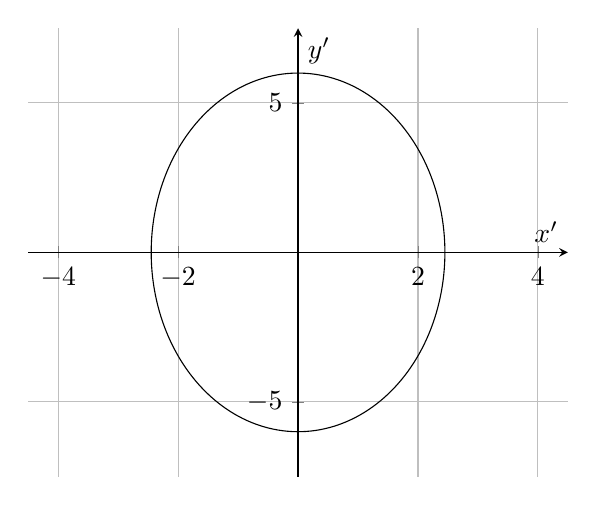
\begin{tikzpicture}
        \begin{axis}[
            axis lines = center,
            grid = both,
            xmax = 4.5,
            xmin = -4.5,
            ymax = 7.5,
            ymin = -7.5,
            xlabel=$x'$, ylabel=$y'$
        ]
        \addplot[
            domain=0:2*pi,
            samples=200,
        ]
        ({sqrt(6)*cos(deg(x))}, {6*sin(deg(x))});
        \end{axis}
    \end{tikzpicture}

\end{solution}